%!TEX root = ../aamas11storage.tex
%%%%%%%%%%%%%%%%%%%%%%%%%%%%%%%%%%%%%%%%%%%%%%%%%%%%
\section{Modular Battery Controller}\label{sec:introduction}
%%%%%%%%%%%%%%%%%%%%%%%%%%%%%%%%%%%%%%%%%%%%%%%%%%%%

Energy storage enables increasing levels of renewable energy in our electricity system, and the rapidly maturing supply chains for several battery technologies encourages electricity utilities, generators, and customers to consider using large battery systems. 

Consider the example scenario of a smart office building comprising of a set of loads (appliances in the building), some renewable sources (solar panels on the roof and a local wind turbine), and a modular battery system. The building is connected to the main grid, and the economics govern that the grid power consumption of the building be maintained within the range $[p_l:p_h]$. Since there is little control over the demand in the building and certainly no control over the renewable generation, then for some period in the day it is possible that the power consumption of the building will fall outside this range. For instance, if the renewable generation is higher than the demand, then the consumption will be negative. Similarly, if the demand is higher than the renewable generation then the building consumption may rise above $P$. In Figure \ref{fig:usecase} the Building Demand plots the sum of consumption and renewable generation in the building and has this property for the period prior to time $t_1$ and after time $t_2$. While this net building demand is fixed all all practical purposes, we do have full control over the use of the battery system. By suitably ordering the battery system to charge (act as a load) or discharge (act as a generator) at determined rates through this period we may influence the net demand in the building. Figure \ref{fig:usecase} shows how the appropriate battery response (Battery Charge) added to the net building consumption (Building Demand) ensures that the power drawn from the grid (Grid Supply) is maintained within the desired range $[p_l:p_h]$.

\begin{figure}[ht]
\begin{center}
%!TEX root = ./dp7-application.tex
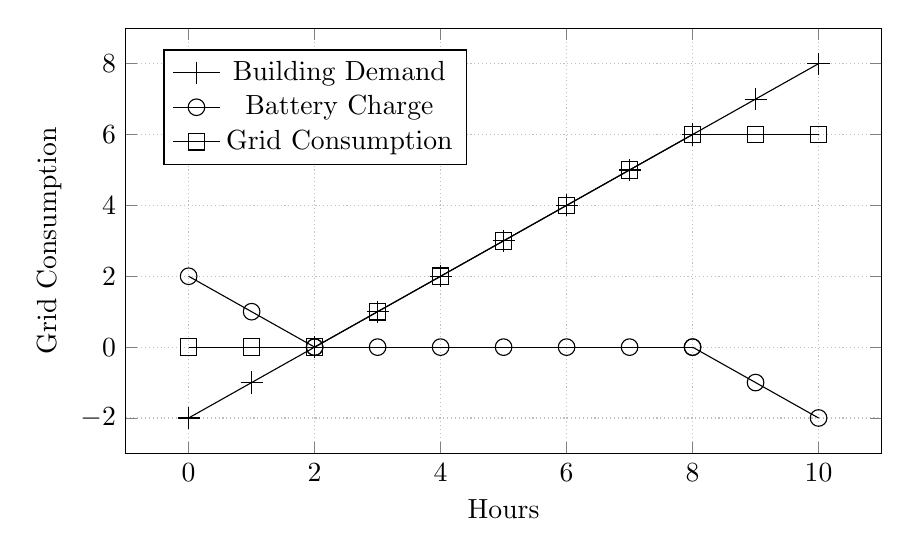
\begin{tikzpicture}

\begin{axis}[
x=0.8cm,y=0.45cm,
xlabel=Hours,
ylabel=Grid Consumption,
grid=both, grid style={style=densely dotted},
legend style={at={(0.05,0.95)},anchor=north west}
] 

% Draw the Demand-Supply curve
\addplot[mark=+,mark size=4] expression[domain=0:10,samples=11] {x-2};
\addlegendentry{Building Demand} 

% Draw the Battery curve
\addplot[mark=o,mark size=3] expression[forget plot,domain=0:2,samples=3] {2-x}; 
\addplot[mark=o,mark size=3] expression[forget plot,domain=2:8,samples=7] {0}; 
\addplot[mark=o,mark size=3] expression[domain=8:10,samples=3] {8-x}; 
\addlegendentry{Battery Charge} 

% Draw the Grid supply curve
\addplot[mark=square,mark size=3] expression[forget plot,domain=0:2,samples=3] {0}; 
\addplot[mark=square,mark size=3] expression[forget plot,domain=2:8,samples=7] {x-2}; 
\addplot[mark=square,mark size=3] expression[domain=8:10,samples=3] {6}; 
\addlegendentry{Grid Consumption} 
\end{axis} 
\end{tikzpicture} 

\end{center}
\caption{Use case scenario for a modular battery system.}
\label{fig:usecase}
\end{figure}

Large battery systems usually comprise of multiple modules and in many installations these may be controlled independently.  Modules may be operated in synchrony but often there are strategic reasons to keep some modules in a different state to others.  For example, if it is undesirable to change the direction of power flow between charging and discharging too frequently, a subset of modules may be used for each direction until it is necessary to change their roles.  Also, some technologies have specific requirements, such as the zinc-bromine flow battery for which a complete discharge at regular intervals is desirable to ``strip'' the zinc plating and ensure irregularities never have an opportunity to accumulate.  Where they exist these requirements place further constraints on module control.

Given, then, an input signal which is the requested rate of charging and discharging for a large battery installation as a function of time, we would like a control algorithm for the set of component modules that implements the requested rate as the sum over the module rates of charging and discharging.  While hardwired control of the battery response is possible, it is often not ideal since the module chemistry is susceptible to change over time and will often cause the battery system performance to diverge from normal. What is needed is adaptable control that accounts for such drift, and as such, a  machine learning approach may be appropriate. 
%The input signal will be different every day but will have many features that are diurnal or nearly so, due to typical variations of electricity demand and solar and wind energy generation sources, and the repetitive patterns that may be seen over several days of the input signal suggest that a learning algorithm may be appropriate.  Our problem is to develop a method for on-line learning that will result in a useful control regime for a modular battery system, when installed at a new site and provided with an input signal derived from the electricity demand and renewable supply at that site.

\begin{figure*}[ht]
\begin{center}
%!TEX root = ../ijcai11storage.tex
\begin{tikzpicture} [level distance=5.5em,child anchor=north]
\tikzstyle{planbox}=[draw,fill=white,text width=5.1em,rectangle split,rectangle split parts=3]
\tikzstyle{goalbox}=[draw,rounded corners=1.25em,minimum height=3em,minimum width=3em]

	
\tikzstyle{level 1}=[sibling distance=6.5em] 
\tikzstyle{level 2}=[level distance=5.5em] 

\node[goalbox,solid] {$G($r,k,s$)$}
	child {node[planbox] {$\pSetCharge$ \\
			\nodepart{second} $k>0$ \\ $\cSatisfies_{ch}(r,k,s)$
			\nodepart{third} $\aSet(k,+c)$
		}
		child {node[goalbox] {$G($r,k-1,s'$)$}}
	}
	child {node[planbox] {$\pSetDischarge$ \\ 
			\nodepart{second} $k>0$ \\ $\cSatisfies_{dc}(r,k,s)$
			\nodepart{third} $\aSet(k,-c)$
		}
		child {node[goalbox] {$G($r,k-1,s'$)$}}
	}
	child {node[planbox] {$\pSetNotUsed$ \\
			\nodepart{second} $k>0$ \\ $\cSatisfies_0(r,k,s)$
			\nodepart{third} $\aSet(k,0)$
		}
		child {node[goalbox] {$G($r,k-1,s'$)$}}
	}
	child {node[planbox] {$\pExecute$ 
			\nodepart{second} $k=0$
			\nodepart{third} $\aOperate()$ \\$\aEvaluate()$
		}
	}
;

\end{tikzpicture}



\end{center}
\caption{Goal-plan hierarchy for the battery system with $k$ modules.}
\label{fig:gptree}
\end{figure*}


%%%%%%%%%%%%%%%%%%%%%%%%%%%%%%%%%%%%%%%%%%%%%%%%%%%%
\subsection{System Design}\label{subsec:design}
%%%%%%%%%%%%%%%%%%%%%%%%%%%%%%%%%%%%%%%%%%%%%%%%%%%%

Figure \ref{fig:gptree} shows a BDI controller for a battery system with $k$ modules. At the beginning of each period of deliberation, the environment posts the top-level goal $G(r,k,s)$. The controller then responds by operating the battery system for that period in a suitable operational state that resolves the goal. Here $r$ specifies the desired response from the battery system and lies in the normalised range $[-1.0:+1.0]$ where $-1.0$ indicates a maximum discharge rate (where all modules are discharging) and $+1.0$ indicates a maximum charge rate (where all modules are charging). The parameter $s$ represents the current state of the battery system, and is derived from sensor readings of each modules current charge and operational state, and $k$ is initially set to the number of modules in the system. 

The resolution of the battery system decides how closely it can match the desired response and is determined by the number of modules $n$. For simplicity, we will assume homogeneous capacity of the modules (but with possibly different chemical properties and constraints), such that each module has a normalised capacity $c$ and $c*n=1.0$. Each module in turn may be configured in one of three states: charging (i.e $+c$), discharging (i.e. $-c$) or not in use (i.e. $0$). The sum of these values gives the net response of the system. By appropriately setting each modules operational state then, the response of the battery system may be adjusted in the range $[-1.0:+1.0]$ in steps of $\pm c$.

The BDI controller works by recursively setting the operational state of each module using the respective $Set*$ plans, and then finally executing the resulting battery configuration for one period and evaluating the result using the $Execute$ plan. The execution therefore always consists of the selection of $k$ high level $Set*$ plans followed by the $Execute$ leaf plan. Using the BDI learning framework from \cite{Singh:RAS10} the pass/fail result is then recorded in the chain of active plans for that period. By training over the outcomes of plan selections in each situation, the system over time learns correct plan selection at each recursive level for the set of possible top-level requests. 

Each plan in the goal-plan hierarchy is further explained below:

$SetCharge$: Set the operational state of module $k$ to {\em Charge} (i.e $+c$) for this period. The plan's context condition first checks that the internal constraints of module $k>0$ will not be violated by this operation. If a violation is expected, then the plan is discarded, otherwise the state is updated and Goal $G$ reposted for module $k-1$.

$SetDischarge$: Set the operational state of module $k$ to {\em Discharge} (i.e $-c$) for this period. The plan's context condition first checks that the internal constraints of module $k>0$ will not be violated by this operation. If a violation is expected, then the plan is discarded, otherwise the state is updated and Goal $G$ reposted for module $k-1$.

$SetNotUsed$: Set the operational state of module $k$ to {\em NotUsed} (i.e $0$). This means that the module will remain disconnected from use for this period. The plan's context condition first checks that the internal constraints of module $k>0$ will not be violated by this operation. If a violation is expected, then the plan is discarded, otherwise the state is updated and the Goal $G$ reposted for module $k-1$.

$Execute$: The leaf plan that actually performs the operations on the battery modules. The plan executes only when $k=0$ which implies that all modules have been configured. All battery modules are then operated simultaneously for this period according to their assigned states. At the end of the period, the plan will evaluate the net battery response against the request. From a learning perspective, the battery response is deemed successful only if it was within tolerance of the desired response, otherwise it is deemed failed.

A $Set*$ plan may be discarded from consideration if the respective constraints for module $k$ are not satisfied for that period. For instance, plan $SetCharge$ may be discarded because module $k$ is only allowed to change charge directions once every four periods say, and charging it in this period will violate that constraint. Similarly, plan $SetDischarge$ may be discarded because the module may already be discharged and further discharge is not possible. 

Since constraint checking is performed in the context condition of the plan i.e. prior to taking any action in the plan body, then BDI failure recovery may be employed to select different $Set*$ plans until all internal constraints are satisfied. Note that failure recovery is not allowed for the $Execute$ plan because it runs for a full period and that is the limit for the decision making. In other words, only one try is allowed per period. So functionally, the $Execute$ plan must always succeed, even though the evaluation against the goal (for learning purposes) may differ.

Finally, the system only learns a response to the immediate request i.e. how to resolve the top level goal. It does not learn any temporal relationship in the sequence of top level goals. For instance, the input signal may have some diurnal or seasonal pattern, however the proposed system does not attempt to learn this pattern. This is perfectly acceptable since the time-scale for decision making (in the order of seconds) is very short compared to the frequency of the pattern.

%%%%%%%%%%%%%%%%%%%%%%%%%%%%%%%%%%%%%%%%%%%%%%%%%%%%
\subsection{On Programmed vs Learnt Behaviour}\label{subsec:constraints}
%%%%%%%%%%%%%%%%%%%%%%%%%%%%%%%%%%%%%%%%%%%%%%%%%%%%

As far as learning systems go, the controller described so far is deployable and will over time learn to configure the battery for any given request - but it is far from ideal. As described later in our experimental setup, the state space for even a $5$-module battery system is quite large (in the order of $13$ million), and will require substantial time to learn. However, before we address the issue of state space we should explain how our learning problem differs from the typical learning scenario.

The problem we are trying to address is that of writing adaptable programs that take into account future changes in the environment. From the outset this means that we want to build a fully functional system based on the current specifications, but one that is capable of adapting (through learning) when the world changes in some predictable way. For instance, in our application, the task is to program a functional controller using the data sheets of the battery modules. However, given the fact that battery performance degrades over time (in a non-deterministic way based on a range of environmental and usage conditions), then we want to program for this future change. 

In some way, we want to start with a program that captures the full set of ideal solutions, but learns to adjust this set based on future changes in the environment. Ideally, the program should cater for additions and subtractions of solutions over time, however for simplicity, we will only consider subtractions in this application. That is to say that we will program our controller with an ideal solution set based on the specifications of the modules, and will allow for future changes that result in solution sets that are subsets of this ideal set. For a battery system this is acceptable since we generally expect batteries to perform `less' over time than at the beginning.

We do this by augmenting {\em operational} constraints into the context condition of the $Set*$ plans. Put simply, operational constraint checking decides if a configuration is admissible given the desired response, the configurations committed to so far, and the number of modules yet to be configured. For instance, a request of $+1.0$ is only serviceable when all modules are configured to charge. So, if module $k$ were to not charge (it may already be fully charged so further charging is not possible), then the operational constraint for module $k+1$ will fail and all $Set*$ plan will fail their context conditions and subsequently be discarded. The ``bad'' configuration of module $k$ makes further configuration pointless, because regardless of how the remaining modules ($>k$) are configured, the response is bound to fall short of the request. When this happens during deliberation, BDI failure recovery allows us to backtrack up the chain of active $Set*$ plans and choose a different path until all constraints are met. Since the $Execute$ plan is run only with configurations that should work (i.e. the ideal solution set), then the system works perfectly i.e. the evaluation against the request always produces a success. However, the important point is that some useful learning still takes place even if the system is always operating the battery correctly. This is because ``internal failures'' during deliberation i.e. when bad configuration paths are abandoned for good ones, provide the necessary negative samples to build a correct classifier. The net result is that the system works perfectly while all the time collecting samples and building an incrementally better classifier for the state space experienced so far. 





%%%%%%%%%%%%%%%%%%%%%%%%%%%%%%%%%%%%%%%%%%%%%%%%%%%%
\subsection{Experimental Setup}\label{subsec:setup}
%%%%%%%%%%%%%%%%%%%%%%%%%%%%%%%%%%%%%%%%%%%%%%%%%%%%

All the experiments were conducted for a battery system with {\em five} modules. The current state of each module was defined as a discrete value in the range $[0:3]$ where zero indicated a fully discharged state and three indicated a fully charged state. As well as this, each module also had an assigned configuration for the period that was one of $Charging$, $NotInUse$, or $Discharging$. The number of possible requests were in the range $[-1.0:+1.0]$ in discrete intervals of $1/n$ i.e. $1/5$ giving a total of $11$ possible requests. The full state space for the problem was then $5 \cdot 11 \cdot 4^5 \cdot 3^5$ or $\approx 13.7$ million. However, note that we do not have to learn over the entire state space since the filtering of nonsensical configurations by the plans context conditions reduces the space dramatically.

At the beginning of a learning episode the configuration of each module was reset to $N$. Moreover, the current state of each module was left untouched, as would be the case in the real system, implying that the state space was not uniformly sampled at the start of each episode. Each episode began with a top-level request from the environment. For simplicity the environment only generated satisfiable requests given the state of the battery system, so that a solution always existed for any given request. The outcome of each episode was either no response (no configuration was chosen), or a single invocation of the $Execute$ plan after which the response was evaluated. The operational model was straightforward, so that charging added $+c$ while discharging added $-c$ to the current state of the respective modules, otherwise the states was left unchanged for the period (no charge loss). The tolerance level was set to $0.0$ so that the battery response was deemed successful only when the sum of the configurations matched the request exactly.

The applicability threshold for plan selection was set to $20\%$ so plans with likelihood of success below this value were discarded from the applicable set. The parameters for stability calculation were $k=1$ and $e=0.5$. For the stability-confidence measure, the averaging window used the last five recordings while the weighting factor was set to $0.5$. Finally, each experiment was run five times and the reported results are averages from these runs.

\subsubsection{Experiment One}

In this experiment we model a scenario where battery module capacities deteriorate..

\begin{figure}[ht]
\begin{center}
%!TEX root = ../aamas11storage.tex
\begin{tikzpicture}

\begin{axis}[
width=0.8\columnwidth,height=4cm,scale only axis,
xlabel=Episodes,
ylabel=Success,
every axis y label/.style={at={(-0.12,0.5)},rotate=90,anchor=center}, 
%every axis x label/.style={at={(0.5,-0.15)},anchor=center},
xtick style={-}, ytick style={-},
grid=both,grid style={-,style=densely dotted},
legend style={at={(0.5,0.25)},anchor=north west}
] 

\addplot[-] file {./data/storage1b.CF.tikzdata};
%\addlegendentry{Data} 

\end{axis} 
\end{tikzpicture} 

\end{center}
\caption{Controller performance with module capacity deterioration.}
\label{fig:experiment1}
\end{figure}

\subsubsection{Experiment Two}

In this experiment we model a scenario where some modules malfunction..

\begin{figure}[ht]
\begin{center}
%!TEX root = ../ijcai11storage.tex
\begin{tikzpicture}

\begin{axis}[
width=0.28\columnwidth,height=3cm,scale only axis,
axis line style={-}, xtick style={-}, ytick style={-},
%xlabel=Episodes,
%ylabel=Success,
every axis y label/.style={-,at={(-0.12,0.5)},rotate=90,anchor=center}, 
%every axis x label/.style={at={(0.5,-0.15)},anchor=center},
grid=both,grid style={-,style=densely dotted},
legend style={at={(0.5,0.25)},anchor=north west}
] 

\addplot[-] file {./data/storage2b.CF.tikzdata};
%\addlegendentry{Data} 

\end{axis} 
\end{tikzpicture} 

\end{center}
\caption{Controller performance with multiple module malfunctions over time.}
\label{fig:experiment1}
\end{figure}



%%%%%%%%%%%%%%%%%%%%%%%%%%%%%%%%%%%%%%%%%%%%%%%%%%%%
\subsection{Analysis}\label{subsec:analysis}
%%%%%%%%%%%%%%%%%%%%%%%%%%%%%%%%%%%%%%%%%%%%%%%%%%%%

Impact of applicability threshold: Reduces number of Execute tries by $7\%$ that is substantial when considering battery life. The difference in performance with and without the applicability threshold is not significant.\footnote{Data: Number of calls to $Execute$ averaged over five runs was $40000$ for test storage2 and $37249$ for test storage2b giving a saving of $7\%$.}

Impact of data filtering: Reduces the training set size by an average of $74\%$ across all plans over all repeats of the experiment. The difference in performance with and without data filtering is not significant.\footnote{Data: The average DT instances for all plans over five runs was $12249.40$ for test storage2b and $3145.75$ for test storage2bm giving a saving of $74.3\%$.}

%The system is (purposely) similar in design to the Towers of Hanoi problem of \cite{Singh:RAS10}. In some respects, it is simpler because the solutions are always at recursive depth $k$. Moreover, the non-leaf $Set*$ plans do not have side-effects when they fail and leave the initial state unaltered. Finally, a solution always consists of a single $Execute$ action whereas in the Hanoi problem it consists of possibly several $Move$ actions\footnote{One point of difference is that this is not a universal library where a solution can always be found. For some requests, no solution will be possible given the internal state of the modules.}.

%Nonetheless, the problem captures a real world problem where it is not straightforward to hand-craft a functional hierarchy and where learning is justified. We do not have a solution to begin with. Then, the size of the problem is still significant - the flow battery in CSIRO Newcastle has $10$ internal modules, so with three possible module states that represents $3^{10}=59049$ possible configurations for a given request. Finally, it offers a realistic scenario for re-learning a solution due to significant changes in the environment. For instance, if an internal module were to fail and had to be replaced, then prior learning may no longer work effectively, and the system will have to adjust and re-learn it's response based on the new characteristics of the updated module.
